


\startchapter{Field Data}
\label{chapter:Fieldalt}


While Chapter 3 and Chapter 4 analyzed controlled experiments, one goal of eDNA technology is its usage in the field. To study how eDNA analysis can be used to detect Coho Salmon in the wild, several field studies were conducted. In particular, four streams in British Columbia were studied (steams AAA, BBB, CCC and DDD). Water samples were collected and associated environmental and physical covariates were recorded. The main fish species of interest was Coho Salmon (\textit{Oncorhynchus kisutch}), although we also considered Cutthroat Trout (\textit{Oncorhynchus clarkii}) and Rainbow Trout (\textit{Oncorhynchus mykiss}). Ecofish personnel also took biomass measurements of each of the species caught using electrofishing.  All biomass measurements were obtained using electrofishing, a method that involves using electric current to temporarily shock and stun fish. Researchers recorded the weight of Coho Salmon, Cutthroat Trout and Rainbow Trout and also recorded the overall weight of all fish that were caught.

\vspace{4mm}

The dataset consists of 432 observations. From each of the four streams, distinct sample locations were chosen. For each sample location, sample replicates were taken each of which consisted of eight observations or technical replicates. Hence there were  432/8= 54 sample replicates as each sample replicate consisted of 8 technical replicates. Nine sample replicates were from stream AAA, nine sample replicates were from stream BBB, eighteen of the sample replicates were from stream CCC and the remaining eighteen sample replicates were from stream DDD. The reason eighteen samples were collected from stream CCC and stream DDD is because two distinct reaches in these streams were studied. Nine replicates were chosen from each reach within these two streams. Samples were collected from streams AAA, BBB and DDD in 2017, while samples from stream CCC were collected in 2018. Within each stream, multiple distinct sections of the stream were chosen to take samples from. These distinct sections are referred to in the dataset as sites.

\vspace{5mm}

In this data analysis we considered the possible impact of covariates on TCT measurements. Firstly, we include the total biomass for each species that was caught in the transect (CO.Total.Biomass.g for Coho). We also included the total biomass per meter squared of transect (CO.Biomass.g.m2 for Coho) and total biomass per meter cubed of transect (CO.Biomass.g.m3 for Coho) calculated using the dimensions of the transect. The environmental covariates that we included were water temperature (Water.Temperature.C), pH, flow rate (Transect.Flow.cms), the distance from shore in meters from which the eDNA sample was taken (eDNA.Distance.from.Shore.m) and the depth of water in meters from which the sample was taken (eDNA.Total.Water.Depth.m). Moreover, we included the possibility of interactions between flow rate and all biomass variables.

\vspace{5mm}

We attempt to show that by accounting for common covariates, researchers may save time and obtain comparable estimates of biomass/abundance to those obtained using costly standard sampling methods such as electrofishing.  We highlight the need for continued research into this topic. Results for Rainbow Trout and Cutthroat Trout can be found in the Appendix. In the following pages, we include summary plots for each of the four streams. We include the total biomass of all fish and Coho Salmon caught in each stream and their associated TCT scores for each sample replicate.


\newpage

\section{Streams}

\subsection{Stream AAA}


\begin{figure}[H]
\centering
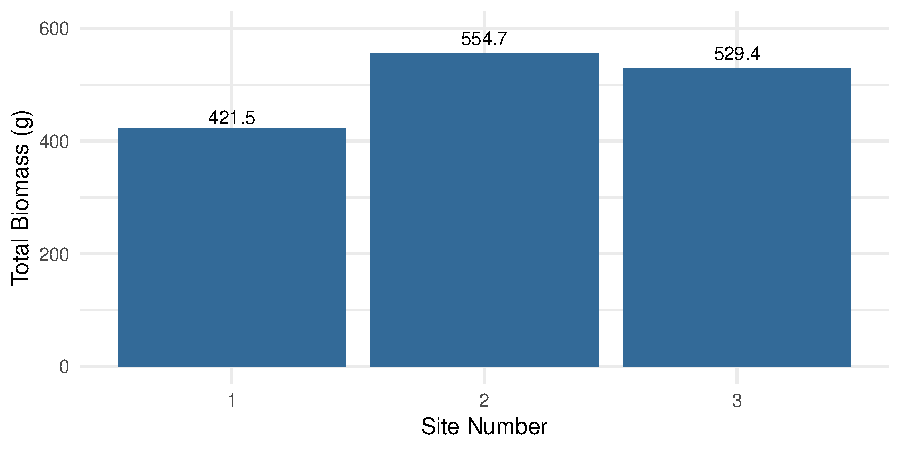
\includegraphics{Chapter5Images/AAA_Ef_new.pdf}
\caption{ Total Biomass for all fish at stream AAA.}
\label{fig:AAA_ef}
\end{figure}



\begin{figure}[H]
\centering
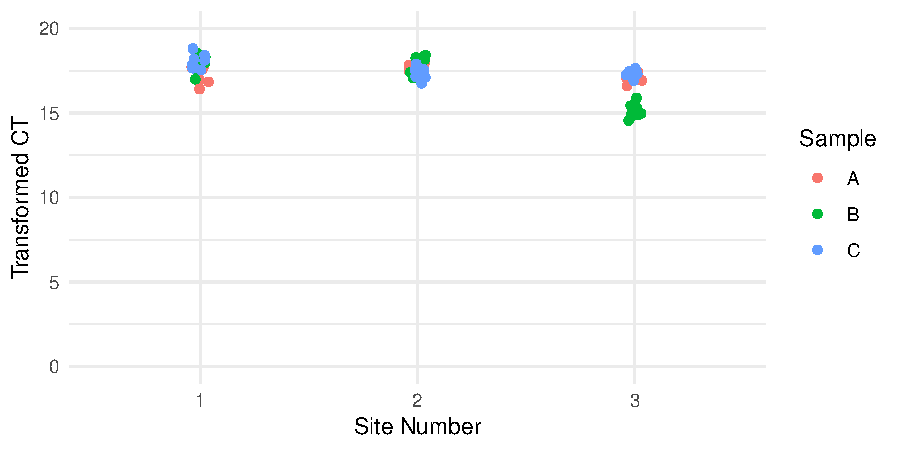
\includegraphics{Chapter5Images/AAA_ef_tct.pdf}
\caption{ Transformed CT values of the technical replicates for all fish at stream AAA.}
\label{fig:AAA_ef2}
\end{figure}






\begin{figure}[H]
\centering
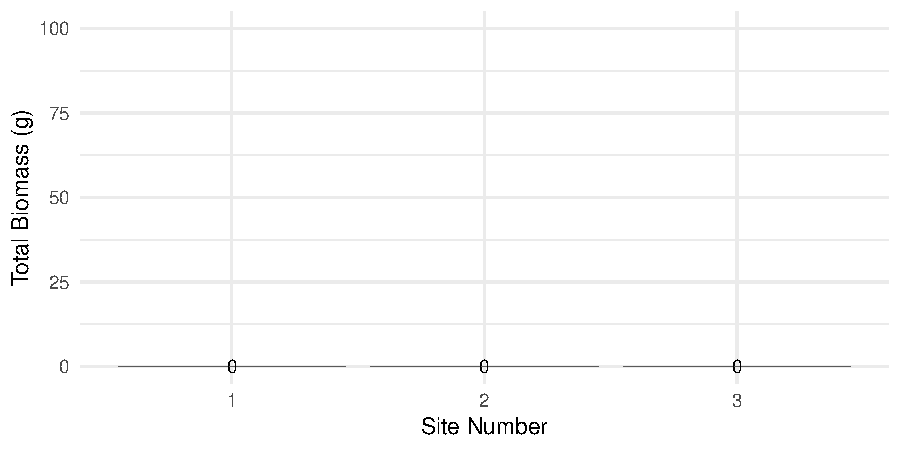
\includegraphics{Chapter5Images/AAA_Co_new.pdf}
\caption{  Total Biomass for Coho Salmon at stream AAA.}
\label{fig:AAA_coho}
\end{figure}



\begin{figure}[H]
\centering
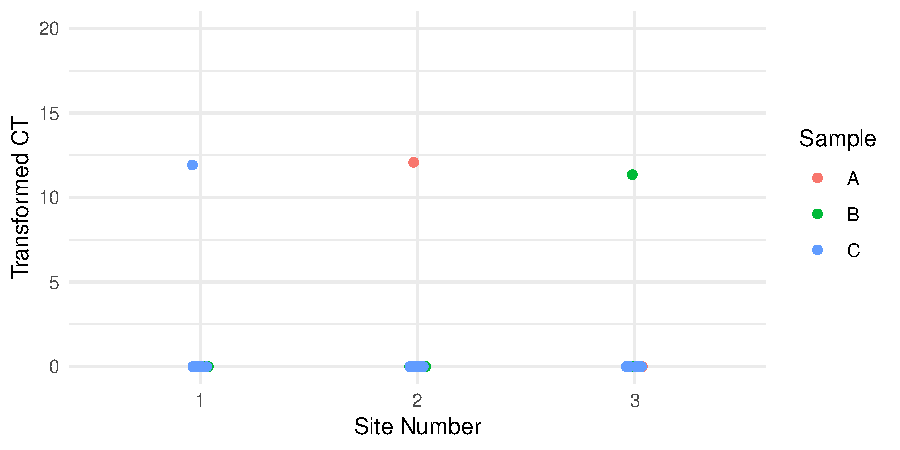
\includegraphics{Chapter5Images/AAA_co_tct.pdf}
\caption{  Transformed CT values of the technical replicates for Coho Salmon.}
\label{fig:AAA_co}
\end{figure}


Figure~\ref{fig:AAA_ef} is a plot of the total biomass for all fish species collected from the three sites at stream AAA. At each site, fish were caught in the transects. Figure~\ref{fig:AAA_ef2} is a plot of the associated TCT values obtained from each site using a primer that amplifies all fish.
\vspace{5mm}
Figure~\ref{fig:AAA_coho} shows that no Coho Salmon were caught at stream AAA. Although Figure~\ref{fig:AAA_co} indicates that there was trace detection of Coho at each of the three sites.


\newpage

\subsection{Stream BBB}



\begin{figure}[H]
\centering
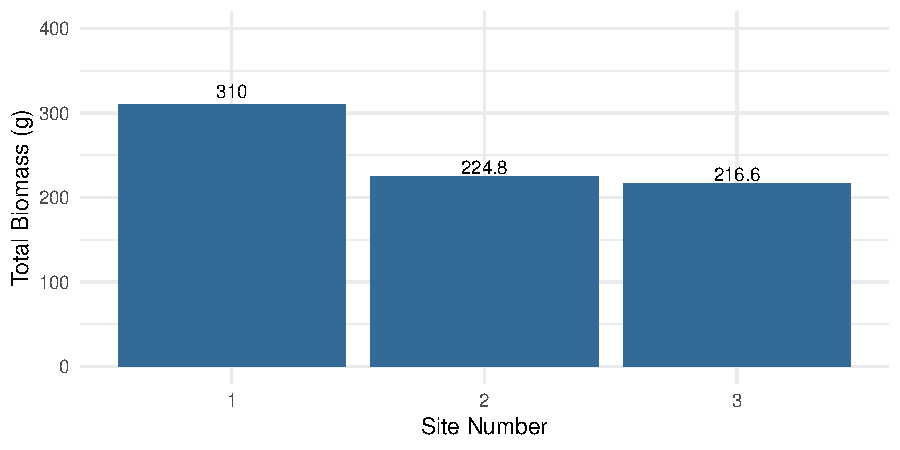
\includegraphics{Chapter5Images/BBB_Ef_new.pdf}
\caption{ Total biomass of all fish at each site for stream BBB.}
\label{fig:testBBBbiom}
\end{figure}



\begin{figure}[H]
\centering
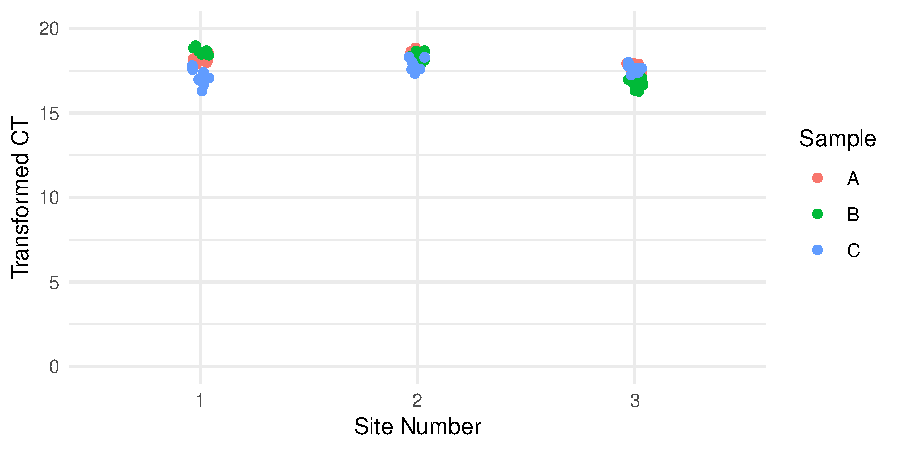
\includegraphics{Chapter5Images/BBB_ef_tct.pdf}
\caption{ Transformed CT values of the technical replicates for all fish.}
\label{fig:BBB_ef}
\end{figure}




\begin{figure}[H]
\centering
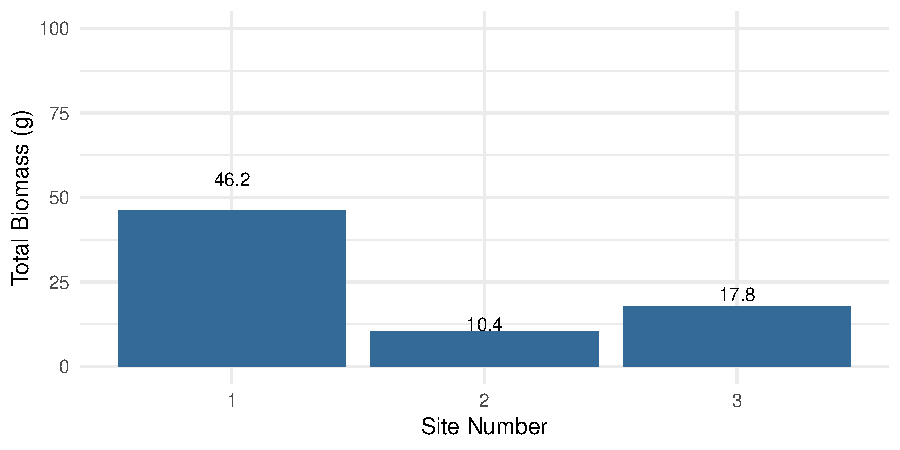
\includegraphics{Chapter5Images/BBB_Co_new.pdf}
\caption{ Total biomass for Coho Salmon at each site for stream BBB.}
\label{fig:testBBBbiomCo}
\end{figure}




\begin{figure}[H]
\centering
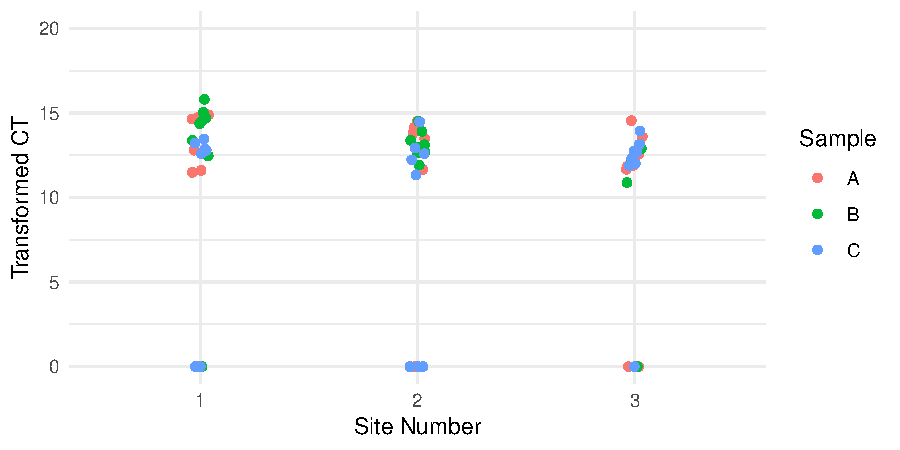
\includegraphics{Chapter5Images/BBB_co_tct.pdf}
\caption{ Transformed CT values of the technical replicates for Coho Salmon.}
\label{fig:BBB_co}
\end{figure}

Figure~\ref{fig:testBBBbiom} is a plot of the total biomass for all fish species collected from the three sites at stream BBB. At each site, fish were caught in the transects. Site number 1 had the highest recorded biomass, although each site had less biomass than those caught in stream AAA. 

\vspace{5mm}

Figure~\ref{fig:BBB_ef} is a plot of the associated TCT values obtained from each site at stream BBB using a primer that amplifies all fish. We see that each site detected relatively high TCT values indicating the presence of fish.

\vspace{5mm}

Figure~\ref{fig:testBBBbiomCo} is a plot of the Coho Salmon that were caught at stream BBB. At each site in stream BBB, Coho were caught. Figure~\ref{fig:BBB_co} confirms the presence of Coho by the moderate TCT values. 

\newpage

\subsection{Stream CCC}




\begin{figure}[H]
\centering
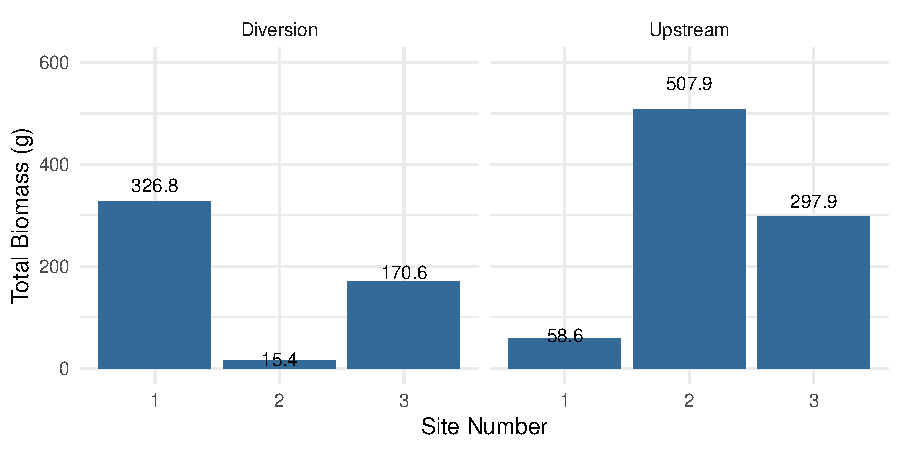
\includegraphics{Chapter5Images/CCC_Ef_new.pdf}
\caption{ Total biomass of all fish at each site for stream CCC.}
\label{fig:testCCCbiomEf}
\end{figure}



\begin{figure}[H]
\centering
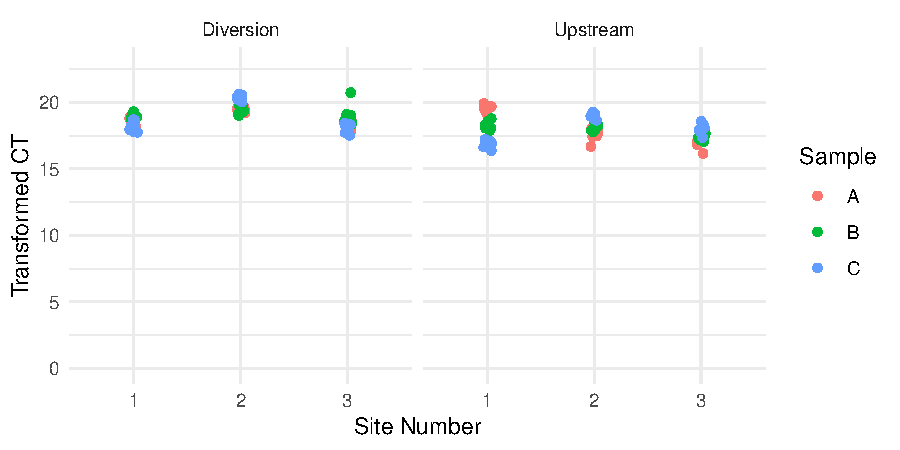
\includegraphics{Chapter5Images/CCC_ef_tct.pdf}
\caption{ \hspace{1mm} Transformed CT values of the technical replicates for all fish.}
\label{fig:CCC_ef}
\end{figure}



\begin{figure}[H]
\centering
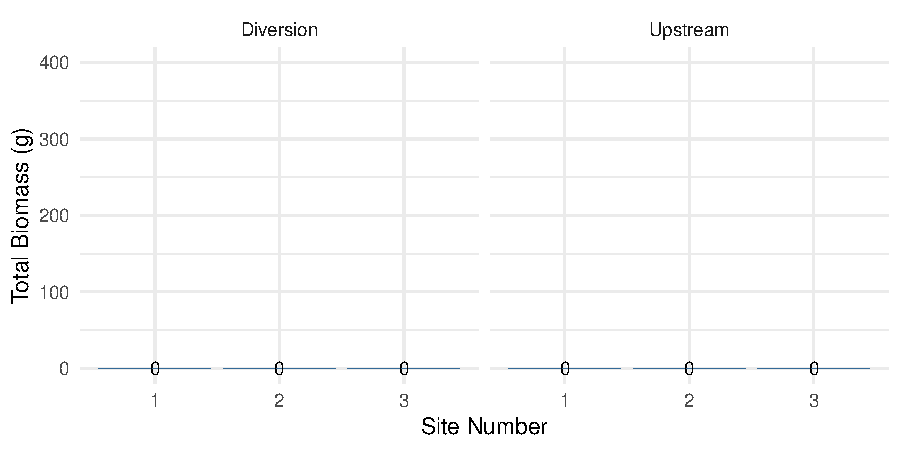
\includegraphics{Chapter5Images/CCC_Co_new.pdf}
\caption{  \hspace{1mm}Total biomass for Coho Salmon at each site for stream CCC.}
\label{fig:testCCCbiomCo}
\end{figure}





\begin{figure}[H]
\centering
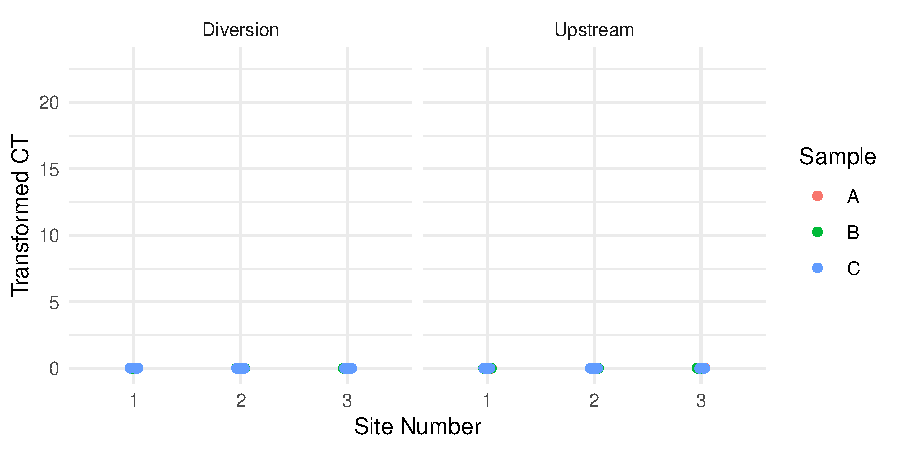
\includegraphics{Chapter5Images/CCC_co_tct.pdf}
\caption{  \hspace{1mm}Transformed CT values of the technical replicates for Coho Salmon.}
\label{fig:CCC_co}
\end{figure}

Stream CCC had two distinct sections, a diversion and a upstream portion. Measurements were thus taken from three distinct sites in each of these distinct portions. Figure~\ref{fig:testCCCbiomEf} shows the biomass of all fish caught at stream CCC. Figure~\ref{fig:CCC_ef} shows the associated TCT values that were obtained from the collected samples.
We see from Figure~\ref{fig:testCCCbiomCo} that no Coho were caught at any portion of this stream. Moreover, Figure~\ref{fig:CCC_co} had no detection of any Coho in any sample.

\newpage

\subsection{Stream DDD}



\begin{figure}[H]
\centering
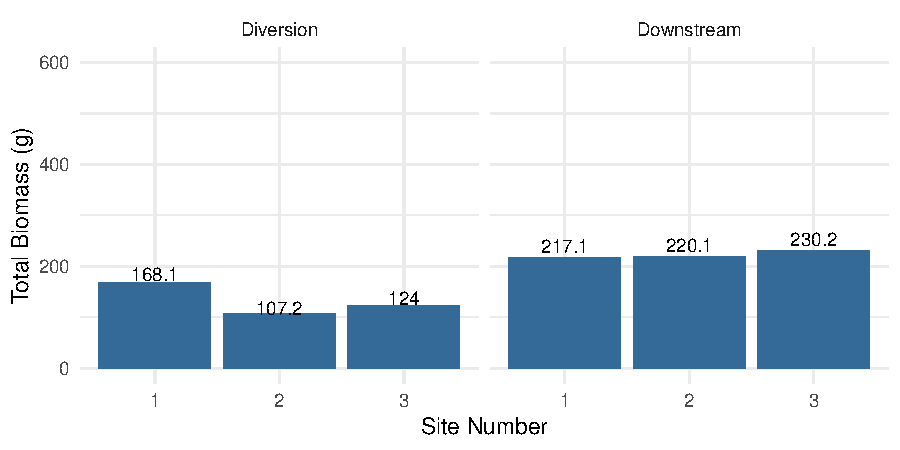
\includegraphics{Chapter5Images/DDD_Ef_new.pdf}
\caption{  \hspace{1mm}Total biomass for all fish at each site for stream DDD.}
\label{fig:testDDDef}
\end{figure}



\begin{figure}[H]
\centering
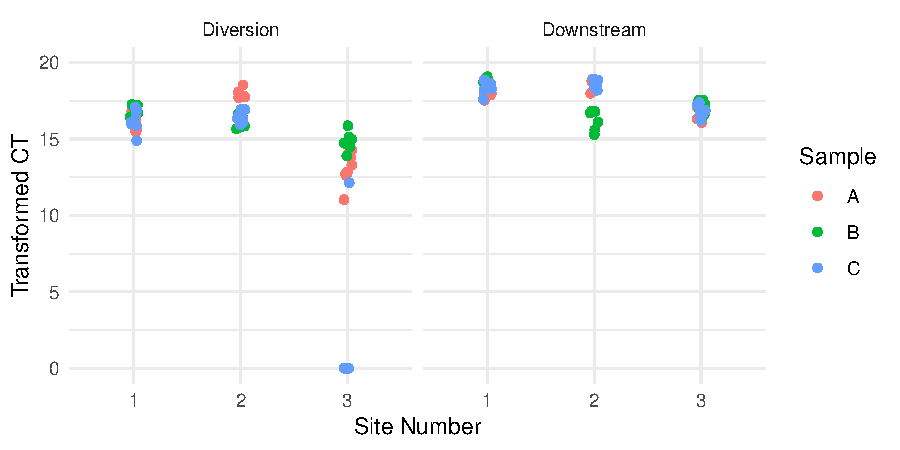
\includegraphics{Chapter5Images/DDD_ef_tct.pdf}
\caption{  \hspace{1mm}Transformed CT values of the technical replicates for all fish.}
\label{fig:DDD_ef}
\end{figure}

\begin{figure}[H]
\centering
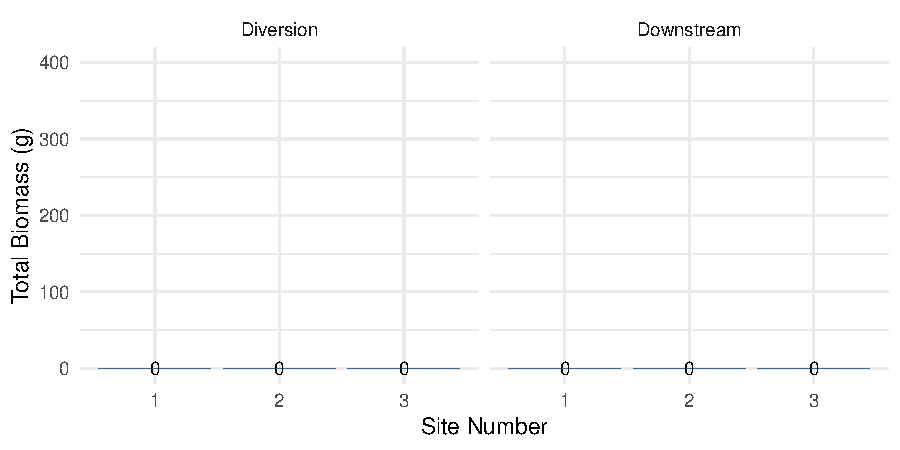
\includegraphics{Chapter5Images/DDD_Co_new.pdf}
\caption{  \hspace{1mm}Total biomass for Coho Salmon at each site for stream DDD.}
\label{fig:testDDDco}
\end{figure}





\begin{figure}[H]
\centering
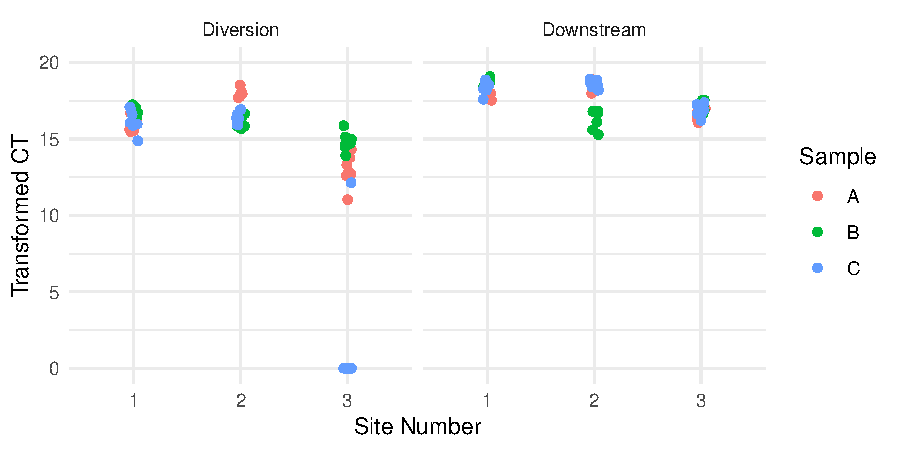
\includegraphics{Chapter5Images/DDD_co_tct.pdf}
\caption{ \hspace{1mm} Transformed CT values of the technical replicates for Coho Salmon.}
\label{fig:DDD_co}
\end{figure}


Stream DDD had two distinct sections, a diversion and a downstream portion. Measurements were thus taken from three distinct sites in each of these distinct portions.
Figure~\ref{fig:testDDDef} shows the biomass of all fish caught at stream DDD. Figure~\ref{fig:DDD_ef} shows the associated TCT values that were obtained from the collected samples.
We see from Figure~\ref{fig:testDDDco} that no Coho were caught at any portion of this stream. However, Figure~\ref{fig:DDD_co} indicates trace detection of Coho Salmon at both the diversion and downstream.



\section{Pairs Plots}



	We now examine how several covariates are associated with one another. We visualize these possible relationships using a `pairs plot'. These plots help illustrate how several variables are possibly correlated. We consider the density and flow terms, as well as previously identified important environmental covariates.  In the case of all fish, one outlier was removed after failing to pass the DNA integrit-E test (this observation was from stream DDD, diversion). The outlier can be seen in the first pairs plot as a blue dot in the bottom left of the first image, in the portion comparing Fish.Total.Biomass.g with MeanTCTEf. The pairs plot compares each predictor with one-another. For example, the first row contains a scatter plot of mean TCT versus each of the other covariates.



\begin{figure}[H]
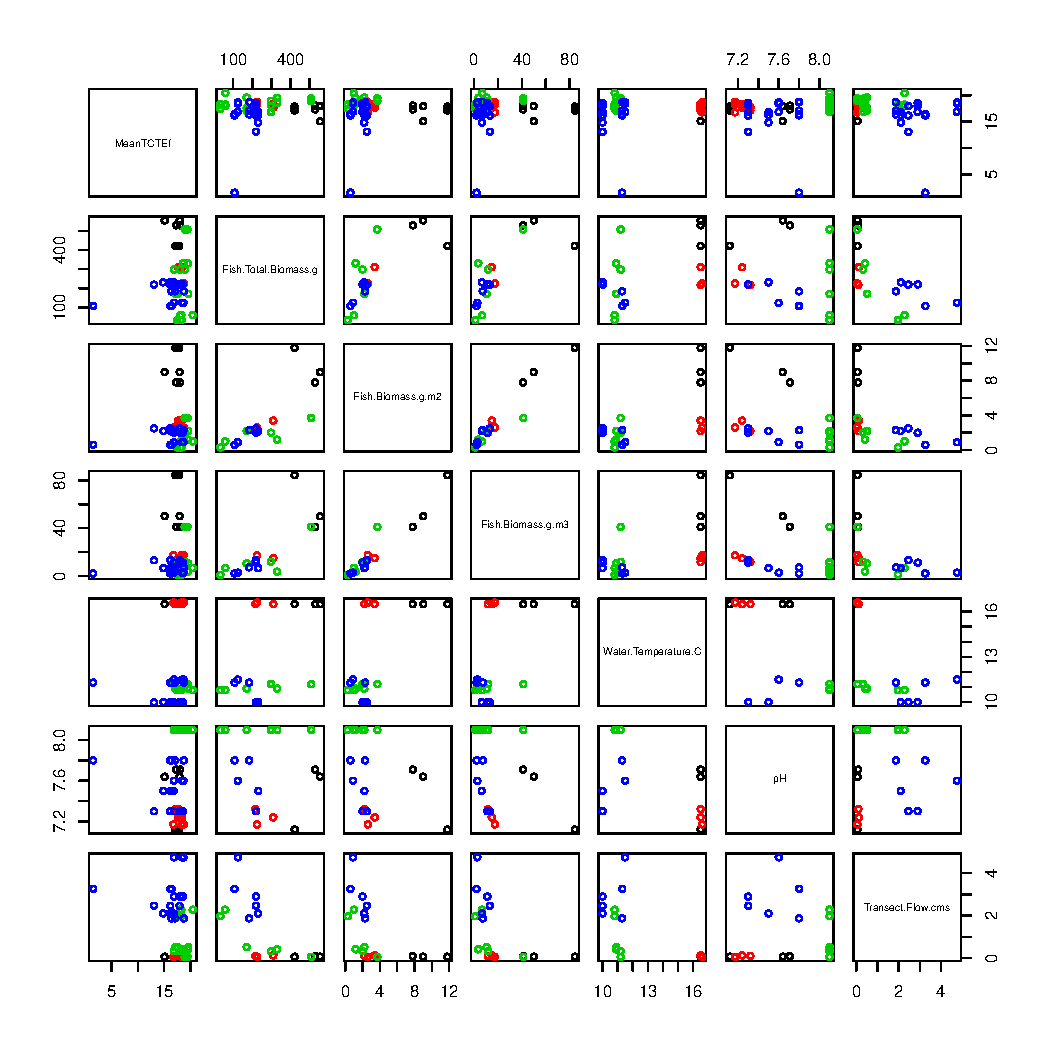
\includegraphics{Chapter5Images/EFishpairs_outlierincluded.pdf}
\caption{  \hspace{1mm}  Pairs plots for all fish with outlier included. We consider several suspected key covariates. Black corresponds to stream AAA, red corresponds to stream BBB, green corresponds to stream CCC and blue corresponds to stream DDD.}
\label{fig:pairefoi}
\end{figure}




\begin{figure}[H]
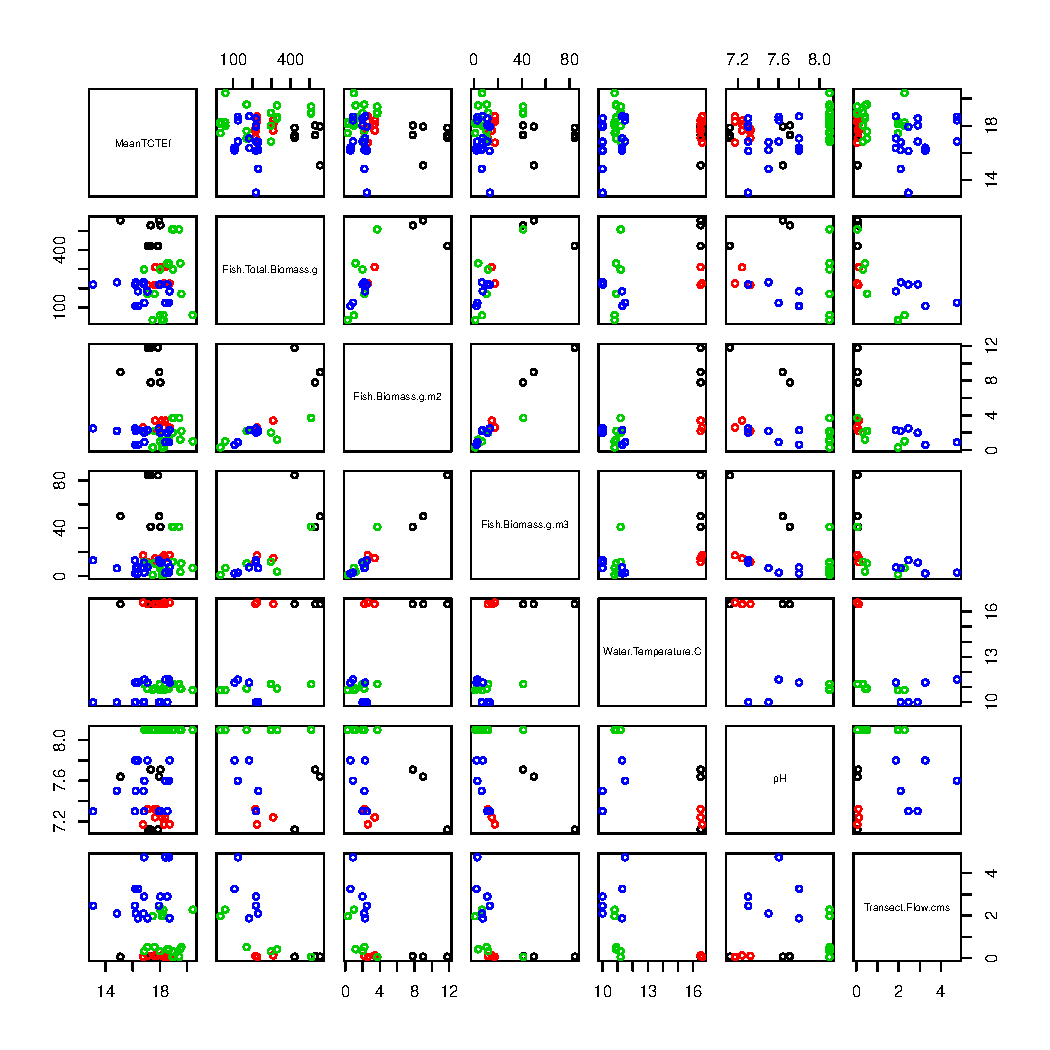
\includegraphics{Chapter5Images/EFishpairs.pdf}
\caption{  \hspace{1mm}  Pairs plots for all fish with outlier removed. We consider several suspected key covariates. Black corresponds to stream AAA, red corresponds to stream BBB, green corresponds to stream CCC and blue corresponds to stream DDD.}
\label{fig:pairef}
\end{figure}


\begin{figure}[H]
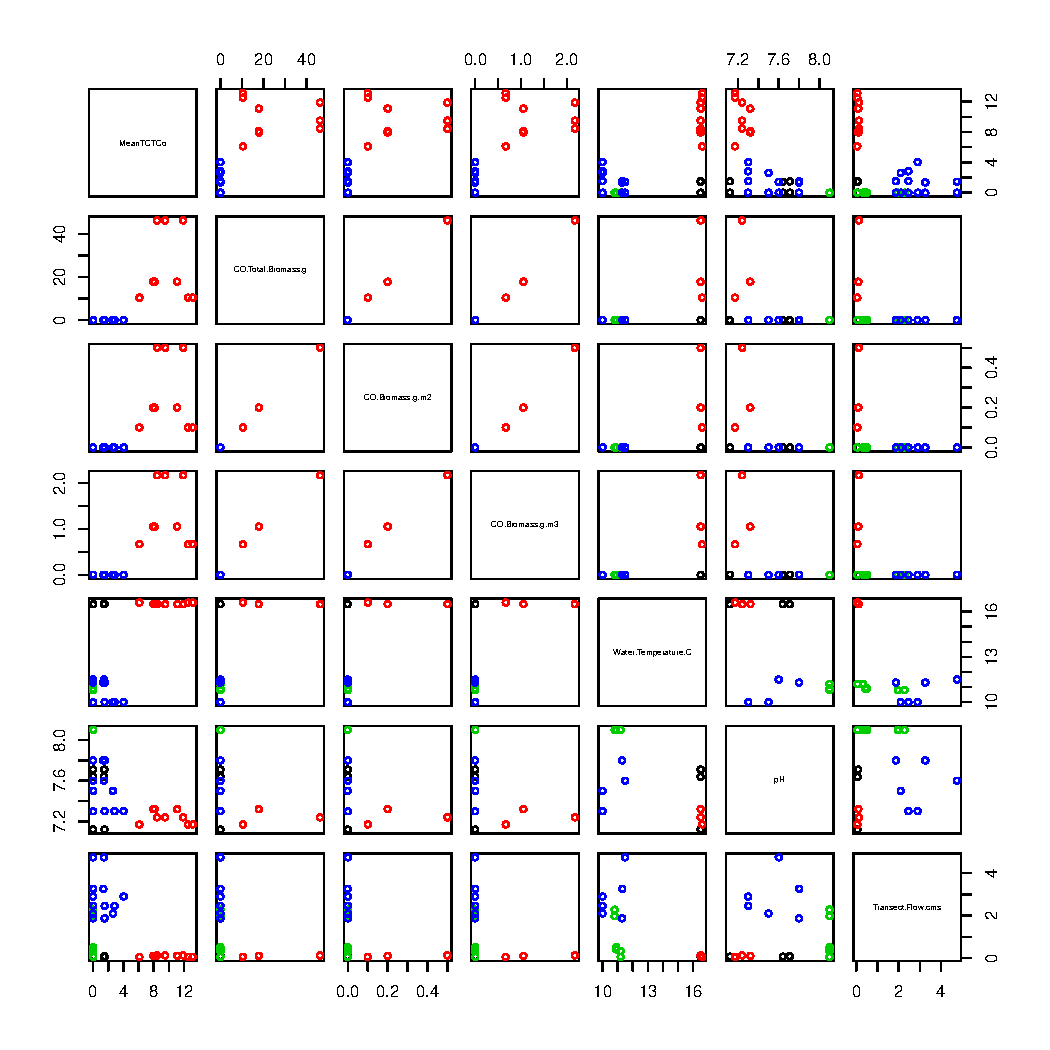
\includegraphics{Chapter5Images/Cohopairs.pdf}
\caption{  \hspace{1mm}Pairs plots for Coho Salmon. Black corresponds to stream AAA, red corresponds to stream BBB, green corresponds to stream CCC and blue corresponds to stream DDD.}
\label{fig:pairco}
\end{figure}

\newpage

The Pairs Plots confirm several of our assumptions. MeanTCT tends to increase linearly as biomass increases. MeanTCT also tends to decrease linearly as Transect.Flow.cms increases. Figure~\ref{fig:pairefoi} is the pairs plot for all fish in which the outlier was included. Figure~\ref{fig:pairef} is the same pairs plot but the outlier from stream DDD diversion was removed. Not much can be analyzed from these plots as there does not appear to be any obvious patterns. However, we see from the colors that samples from the same stream tend to cluster together. Figure~\ref{fig:pairco} is the pairs plot for Coho. We see from observing the first row that MeanTCT appears to increase linearly with CO.Total.Biomass.g, CO.Biomass.g.m2 and CO.Biomass.g.m3. MeanTCT also appears to possibly increase with higher water temperatures (Water.Temperature.C), and possibly decreases with higher levels of pH. MeanTCT also appears to decrease as Transect.Flow.cms increases.



\newpage

\section{TCT versus Biomass}

Although several covariates likely influence mean transformed CT scores, we expect a relationship between biomass and TCT. We visualize this one variable (mean over eight technical replicates) using a simple linear regression model before the addition of covariates.


Firstly, we considered linear models with biomass as the only predictor for Mean TCT.  Biomass refers to the weight in grams of the fish caught in the transect using electrofishing. 

\vspace{3mm}



\begin{figure}[H]
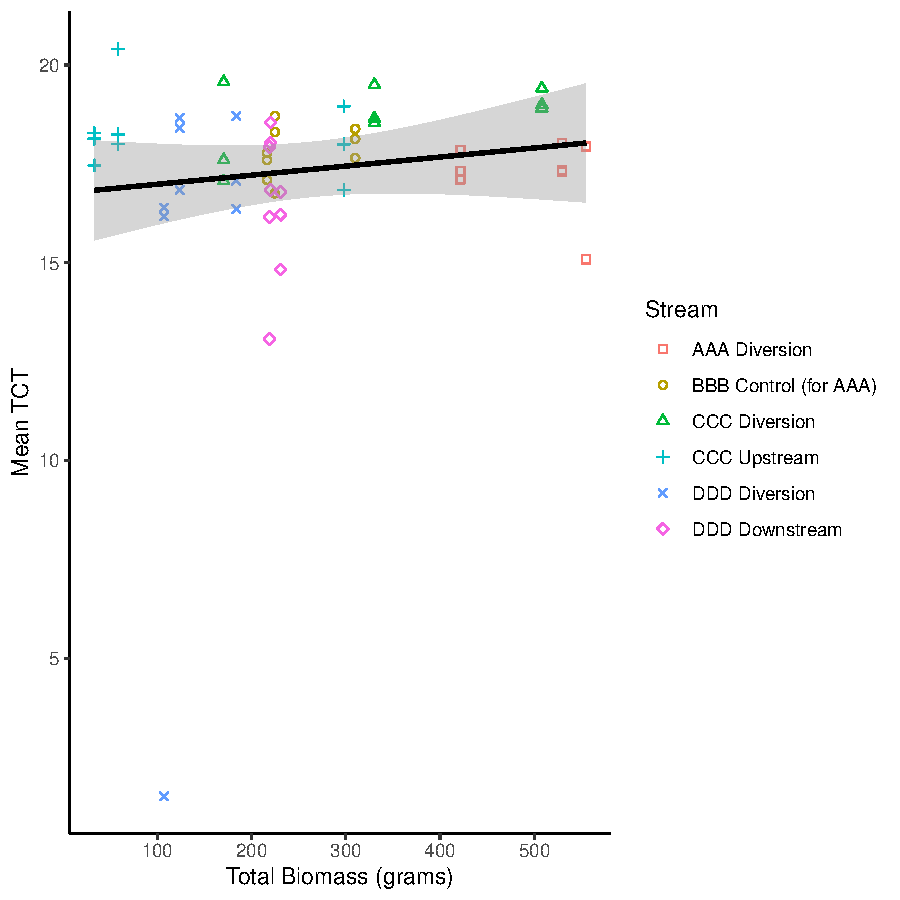
\includegraphics{Chapter5Images/gg_ef.pdf}
\caption{ \hspace{1mm} Mean TCT over each set of eight technical replicates versus Total Biomass for All Fish, outlier removed. Included is the simple linear regression model and the 95\% Confidence limits for the regression line.}
\label{fig:efanalysis}
\end{figure}


\begin{table}[H]
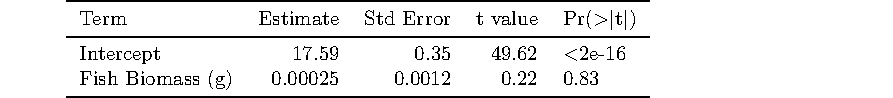
\includegraphics{Chapter5Images/eflinearfield.pdf}
\caption{Parameter estimates and standard errors for a model that considers biomass for all fish. Model: model.fish.}
\label{fig:modelef}
\end{table}


 Figure~\ref{fig:efanalysis} is the plot of the model, model.fish and the associated confidence limits. The line appears flat, and no obvious relationship is clear from a simple visual consideration. Table~\ref{fig:modelef} provides a summary of the simple linear model (model.fish) fit for All Fish. The $R^{2}$ is only 0.00093. Although the estimate for the coefficient of biomass is still positive, the estimate is not statistically significant. 


\begin{figure}[H]
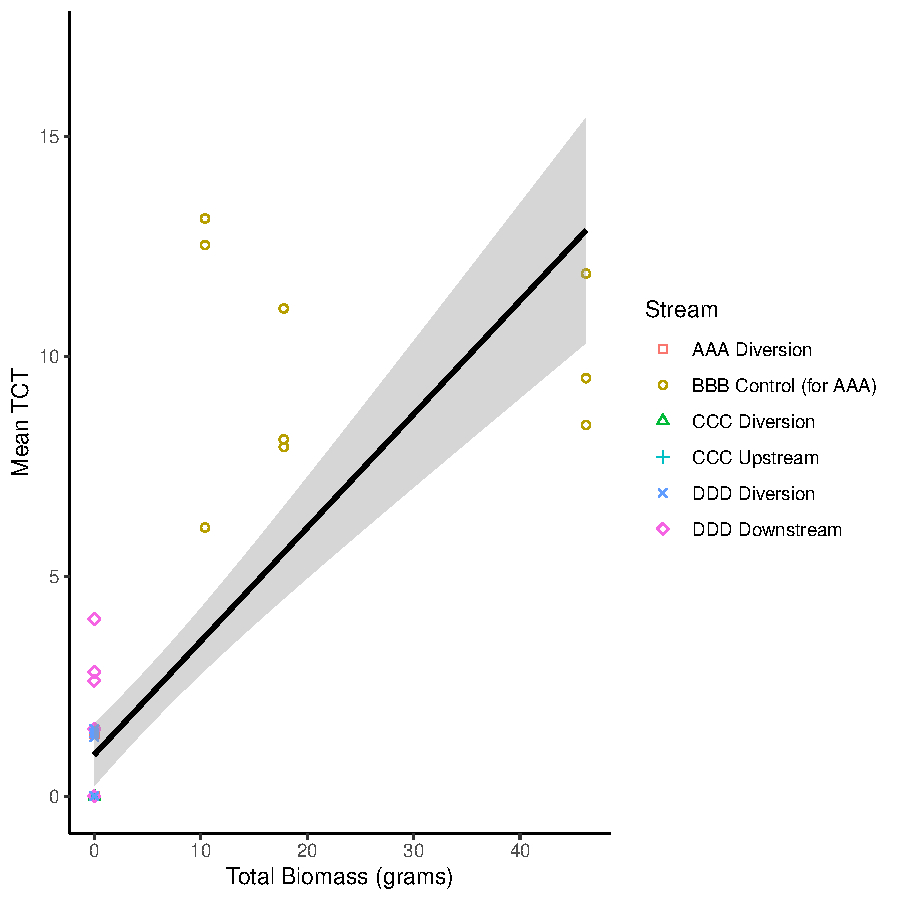
\includegraphics{Chapter5Images/model_CO.pdf}
\caption{  \hspace{1mm}Mean TCT over each set of eight technical replicates versus Total Biomass for Coho Salmon. Included is the simple linear regression model (Biomass as the only predictor) and the 95\% Confidence limits for the regression line.}
\label{fig:cohoanalysis}
\end{figure}


\begin{table}[H]
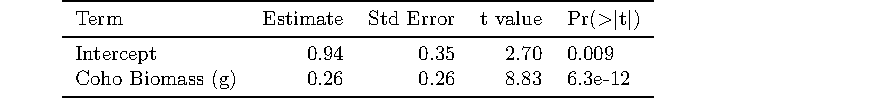
\includegraphics{Chapter5Images/coholinearfield.pdf}
\caption{Parameter estimates and standard errors for a simple linear model for Coho. Model: model.co.}
\label{fig:modelco}
\end{table}



For Coho Salmon, our estimated positive of coefficient of +0.26 on biomass is statistically significant.  Figure~\ref{fig:cohoanalysis} makes the relationship clear. Mean TCT increases as CO.Total.Biomass.g increases. Table~\ref{fig:modelco} provides the summary of the simple linear model for mean TCT for Coho. The simple linear model only considered the predictor CO.Total.Biomass.g and achieved an $R^{2}$ of 0.600



\subsection{Environmental Factors}


We now consider the possible impact of covariates on the Mean TCT value. We include summary statistics of several of those covariates that have been shown to impact eDNA degradation such as pH and water temperature. We also include several biomass related terms such as total biomass, total biomass per meter squared of transect and total biomass per meter cubed of transect. We also include a `flow' term by considering the flow through the transect. 



\begin{table}[H]
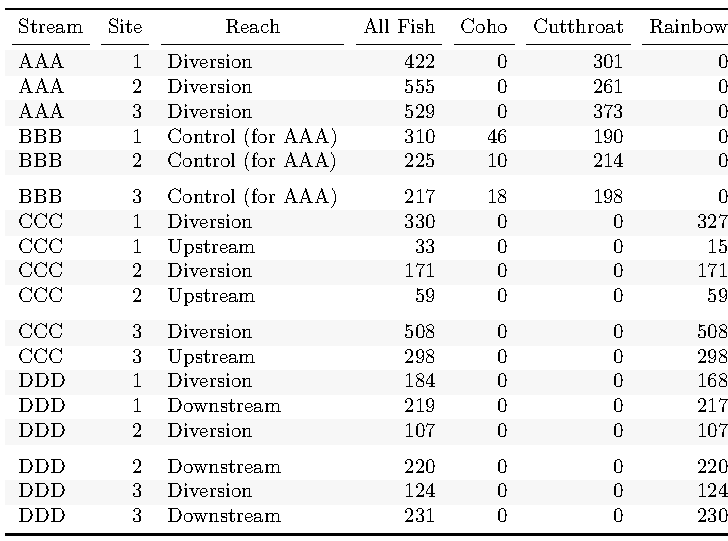
\includegraphics{Chapter5Images/biomass_kable.pdf}
\caption{ \hspace{1mm} Table showing the total biomass (g) of each species captured in the transect for each site.}
\label{fig:kablemass}
\end{table}


Table~\ref{fig:kablemass} summarizes the total biomass of Coho, Cutthroat, Rainbow and all Fish that were caught in the transects in each site at each stream. Coho was only caught in stream BBB.


\begin{table}[H]
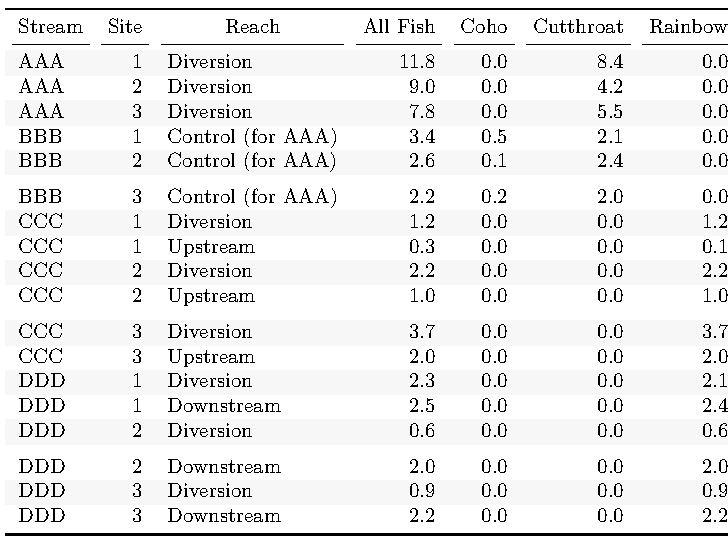
\includegraphics{Chapter5Images/kable_gm2.pdf}
\caption{   \hspace{1mm}Table showing the total biomass (g) of each species captured in the transect per meter squared of transects for each site.}
\label{fig:kablemass2}
\end{table}



\begin{table}[H]
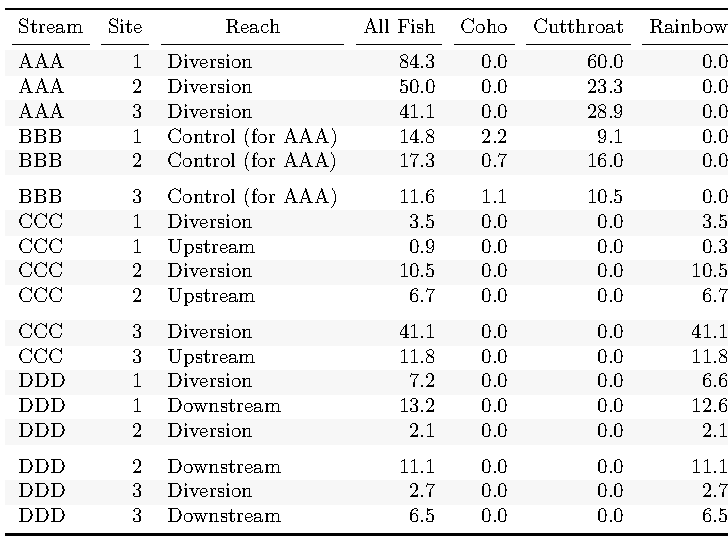
\includegraphics{Chapter5Images/kable_gm3.pdf}
\caption{  \hspace{1mm} Table showing the total biomass (g) of each species captured in the transect per meter cubed of transects for each site.}
\label{fig:kablemass3}
\end{table}





\begin{table}[H]
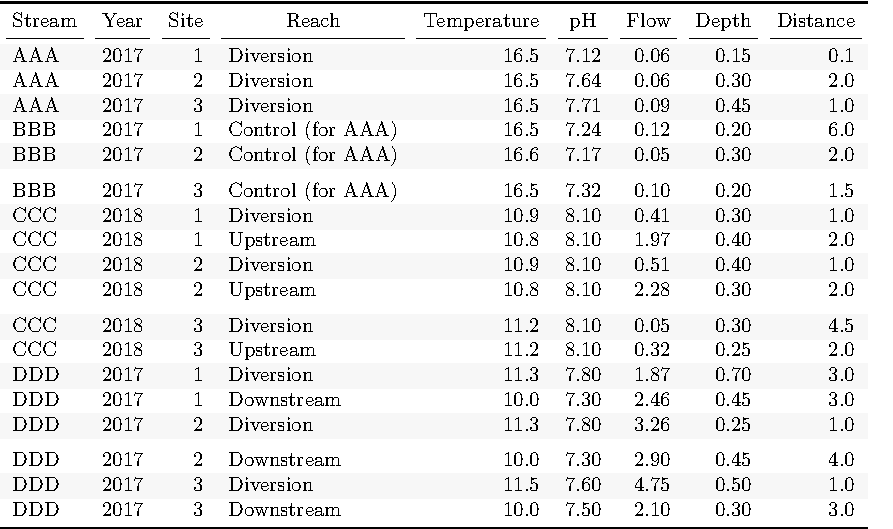
\includegraphics{Chapter5Images/test_update.pdf}
\caption{  \hspace{1mm}  Table showing a variety of summary statistics taken over each site. Temperature is in Celsius, pH is a scale and Transect Flow is in (cm/s), Depth is the depth of the sample area in meters, and Distance is the distance in meters from shore in which the sample was taken.}
\label{fig:kabletemp}
\end{table}

Table~\ref{fig:kablemass2} summarizes the weight of each species caught per meter squared of transect. Table~\ref{fig:kablemass3} shows the weight of each species caught per volume of transect, calculated by using the depth of the transect. The reason that the weight per volume is larger than the weight per area is due to the fact that the transect depth was often very shallow and less than 1 meter. Table~\ref{fig:kabletemp} summarizes a variety of covariates that were recorded at each stream. These environmental covariates are taken into account in our statistical models. 


\newpage

\subsection{Models with Covariates}

To determine a suitable model for mean TCT for Coho we used backward elimination. Other than biomass per meter cubed of transect (CO.Biomass.g.m3), the original covariates that we considered were the water temperature in Celsius (Water.Temperature.C), the pH, the flow rate (Transect.Flow.cms), and the interaction between Transect.Flow.cms and CO.Biomass.g.m3. We also considered sampling covariates such as the sampling depth (eDNA.Water.Sampling.Depth.cm) and the distance from shore in which the sample was collected (eDNA.Distance.from.Shore.m).

\vspace{5mm}

The initial `full' model is named model.coho.full;

\vspace{5mm}

\begin{table}[H]
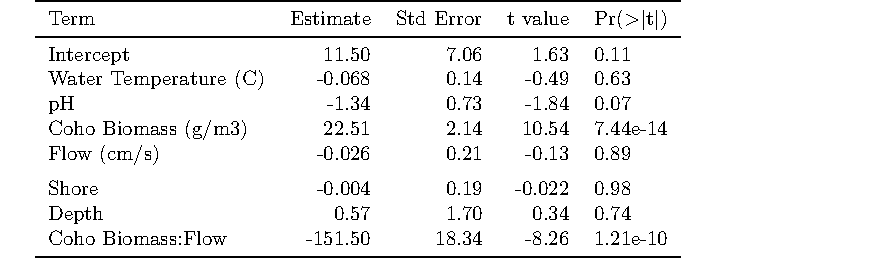
\includegraphics{Chapter5Images/cohofull.pdf}
\caption{Parameter estimates and standard errors for the model.coho.full. The $R^{2}$ for this model is 0.902. }
\label{fig:fullcoho}
\end{table}

Table~\ref{fig:fullcoho} is a summary of the full model, model.coho.full. The fitted model indicates high levels of significance for CO.Biomass.g.m3, and a high significance estimate for the interaction between CO.biomass.g.m3 and Transect.Flow.cms.

\vspace{5mm}

Backward elimination is performed using `stepAIC' \citep{MASS} with the direction argument specified as `backward'. We first feed a full model, with all possible covariates into the algorithm and it proceeds as follows; R determines which predictor (if any) when removed will decrease the AIC the most.  Once R determines that there are no predictors left that can be removed (i.e. there is no predictor that can be removed that results in a decreased AIC), the algorithm terminates. Akaike Information Criteria (AIC) allows us to compare similar models. One method to select a suitable model would be to select the model with the lowest AIC value. Note that this is because $AIC=2*p-2\log(\hat L)$ where p is the number of predictors and $\hat{L}$ is the maximum value of the likelihood function. 
AIC accounts for overfitting by penalizing the addition of more predictors. After comparing three biomass parameters (CO.total.Biomass.g, CO.Biomass.g.m2 and CO.Biomass.g.m3) we decided to work with CO.Biomass.g.m3 as this quantity can be interpreted as a fish `density' parameter. We also include a scope argument to the stepAIC algorithm which ensures that CO.Biomass.g.m3 is always included in the model.




\vspace{5mm}

\begin{table}[H]
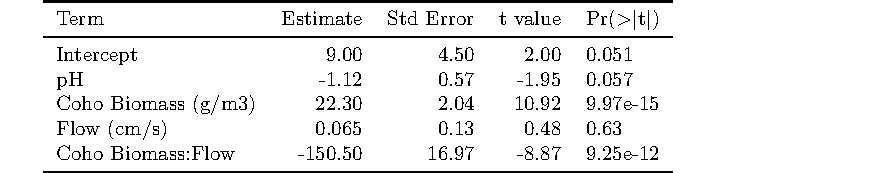
\includegraphics{Chapter5Images/cohored.pdf}
\caption{Parameter estimates and standard errors for the stepwise reduced model, model.co.step. The $R^{2}$ for this model is 0.901.}
\label{fig:cohostep}
\end{table}



For Coho, stepwise selection of covariates indicates we should include several covariates as seen from Table~\ref{fig:cohostep}. CO.Biomass.g.m3 is a significant predictor, as well as the interaction between Transect.Flow.cms and CO.biomass.g.m3. We see as CO.biomass.g.m3, mean TCT also increases.  The interaction between CO.biomass.g.m3 and Transect.Flow.cms indicate that higher levels of flow may result in lower levels of mean TCT, as we have a highly negative estimate for the interaction term. pH also appears to have an impact; whereby higher pH water may result in lower estimates of TCT. By including Transect.Flow.cms and the interactions between Transect.Flow.cms and CO.Biomass.g.m3, we have greatly increased the $R^{2}$ to 0.901 and we have an adjusted $R^{2}$ of 0.893.

\vspace{3mm}

The highly negative estimated coefficient for the interaction can be explained by an examination of Figure~\ref{fig:pairco} and Table~\ref{fig:kabletemp}. The interaction term between CO.Biomass.g.m3 and Transect.Flow.cms . This may imply that larger fish are more greatly impacted by flow. That is, at higher levels of flow, the biomass of a species may become less important in determining mean TCT. Moreover, the large magnitude of the estimate is partially due to the fact that the term Transect.Flow.cms is in units of cm/s.

\vspace{3mm}

Overall, these models indicate the significance of a few key covariates. When attempting to model mean TCT, researchers may wish to first include covariates such as pH and flow rate, as well as possible interactions between the flow rate and biomass. In our analysis, higher levels of Transect.Flow.cms tended to result in lower estimates of mean TCT (likely due to the `washing away' of the eDNA). Higher levels of pH appear to result in lower TCT, possibly due to degradation of eDNA. Researchers may wish to start with a model that includes all predictors of interest and  remove ecological covariates one at time using backward-elimination.

\newpage

\subsection{Model Averaging}


We now explore the concept of  `Model Averaging'. In particular, we make use of the R package `MuMIn: Multi-Model Inference' \citep{mumin}. This package also assists in model selection. MuMIn also provides us with confidence intervals for our parameters.  We use the R function `dredge' to generate a model selection table (ma.coho) using the full model, model.co.full. dredge creates and evaluates multiple subsets of the full global model. Note that `Adjusted AIC' or `AICc' is defined as $AICc= AIC+ \frac{2p^{2}+2*p}{N-p-1}$. Adjusted AIC is often preferred when the sample size, N, is small.


\begin{table}[H]
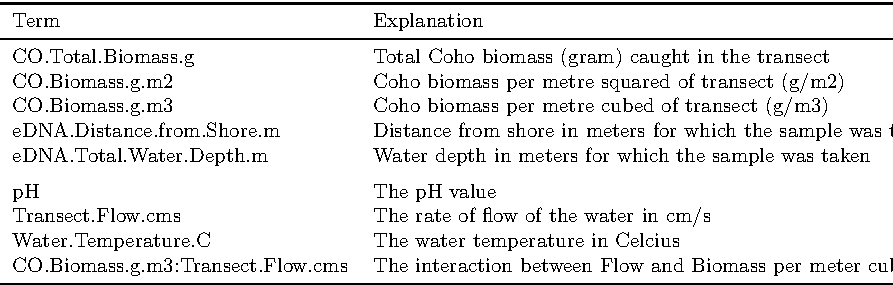
\includegraphics{Chapter5Images/termexp.pdf}
\caption{Explanations for predictors.}
\label{fig:termexp}
\end{table}




\begin{table}[H]
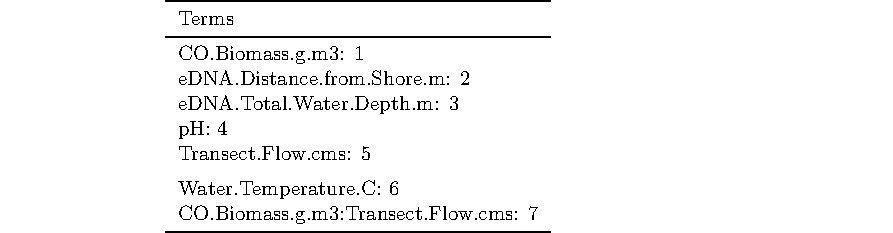
\includegraphics{Chapter5Images/termcodes.pdf}
\caption{Term codes for predictors.}
\label{fig:termcodes}
\end{table}


\begin{table}[H]
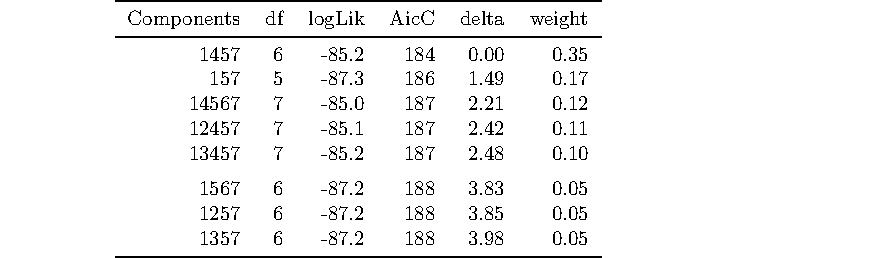
\includegraphics{Chapter5Images/modelAV.pdf}
\caption{Final results for model Averaging. Each model is included with a weight, with stronger models having higher weights. }
\label{fig:modelav}
\end{table}







Table~\ref{fig:termexp} summarizes what each predictor represents. Table~\ref{fig:termcodes} lists the associated term codes that are used in the model averaging. Table ~\ref{fig:modelav} lists the estimates and components for the model average object. The term codes are used to save space and are used as a numeric reference to our predictors. The component models section is a list of the variety of differing models in which we are averaging over. The highest weighted model (with a weight of $w=0.35$) is the model containing CO.Biomass.g.m3, pH, Transect.Flow.cms and the interaction between CO.Biomass.g.m3 and Transect.Flow.cms. This is indeed the same model chosen using backward selection. The next highest weighted model (with a weight of $w=0.17$) is simply the first model but with pH removed. We specify a delta of less than 4. That means R only returns to us component models in which the adjusted AIC does not differ by more than 4. The delta term represents the difference in adjusted AIC each model is from the best model. For example, the second best model which contains CO.Biomass.g.m3, Transect.Flow.cms and CO.Biomass.g.m3:Transect.Flow.cms differs in adjusted AIC from the highest weighted model by 1.49. Our components are thus all combinations of predictors such that the adjusted AIC is within 4 of the best performing model.


\vspace{5mm}



\begin{table}[H]
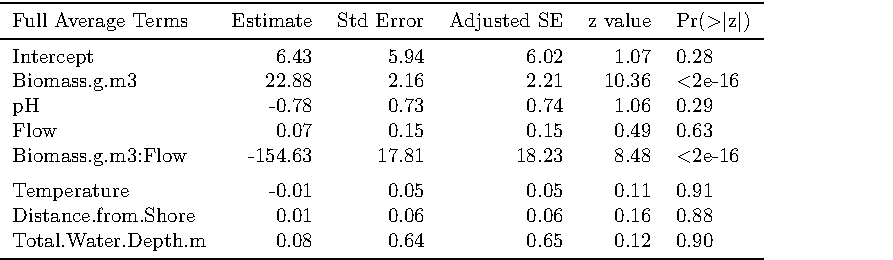
\includegraphics{Chapter5Images/fullAV.pdf}
\caption{Parameter estimates and standard errors for the full model averaging model.}
\label{fig:fullav}
\end{table}

\begin{table}[H]
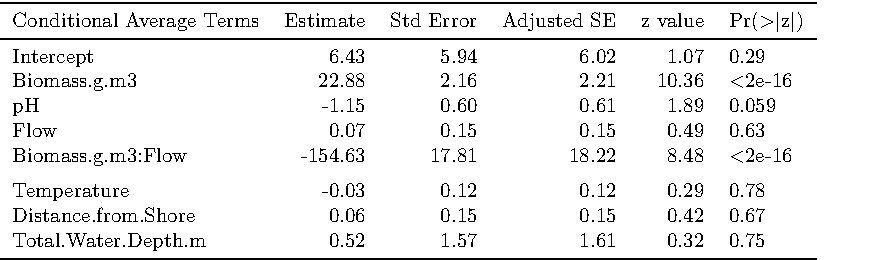
\includegraphics{Chapter5Images/condAV.pdf}
\caption{Coho Model Average Estimates.}
\label{fig:condav}
\end{table}



 MuMIn works by ranking models according to their adjusted AIC. MuMIn reports two tables of estimates. The first estimates (Table~\ref{fig:fullav}) are denoted as `full average' are the estimates obtained via averaging over all possible models (including models in which this predictor is not present. The second set of estimates (Table~\ref{fig:condav}), denoted as `conditional average' are the estimates obtained via averaging over all models in which that predictor is present. The `full' average coefficient considers models that are more than 4 units away in adjusted AIC. 

\vspace{5mm}


\begin{table}[H]
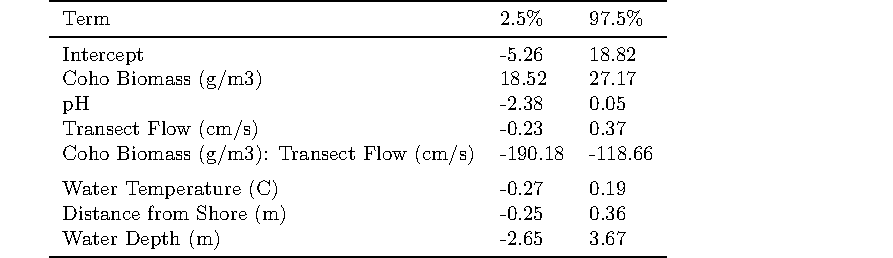
\includegraphics{Chapter5Images/95conf_coho.pdf}
\caption{95\% Confidence Interval for parameter estimates.}
\label{fig:co95}
\end{table}





Table~\ref{fig:co95} lists 95 \% confidence intervals for the coefficient estimates provided by the conditional-average coefficients. The estimates are similar to those obtained using backward elimination.





\newpage

\subsection{Best possible Subset}

We now use the R  `leaps' package \citep{leaps} to compare models using the `Best Subset Method'. This algorithm (regsubsets in R) fits the best possible subset of each subset size. We compare models using three criteria,  `Mallow's Cp' or `Cp', adjusted $R^{2}$, and the Bayesian Information Criterion (BIC).  One could also return the `nbest' models for each subset size if we wished to obtain a list of candidate models.  The BIC is defined as $BIC=log(N)*p-2\log(\hat L)$ where p is the number of predictors, $\hat{L}$ is the maximum value of the likelihood function and N is sample size. The BIC is similar to the AIC; however, it more heavily penalizes complexity compared to the AIC.

\vspace{5mm}

Cp is another model selection metric and is defined as $$Cp=\frac{SSres}{s^{2}}+2(p+1)-N$$ Where SSres is the sum of squared residuals for the linear model fit using p parameters. N is the sample size and $s^{2}$ is an estimate of the Mean Squared Error.

\vspace{5mm}

 \begin{singlespace*}
\fontsize{11pt}{12pt}\selectfont
\verbatiminput{Chapter5Images/subsets_coho.txt}
\end{singlespace*}


\begin{table}[H]
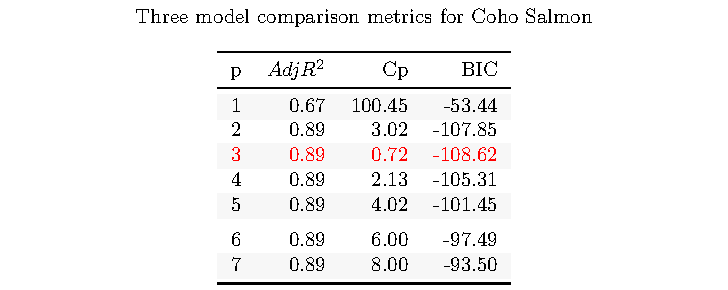
\includegraphics{Chapter5Images/subsets_kable.pdf}
\caption{ Table summarizing model comparison metrics for Coho Salmon. The red indicates the chosen model according to the lowest BIC.}
\label{fig:cohocompare}
\end{table}

\begin{table}[H]
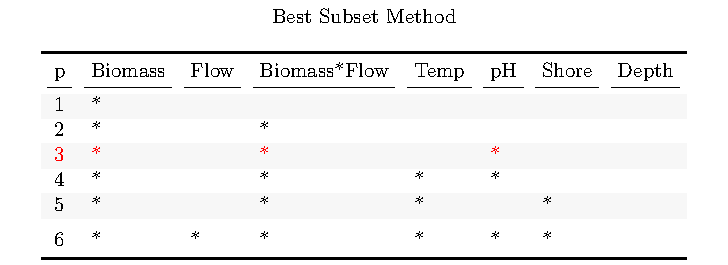
\includegraphics{Chapter5Images/best_subredo.pdf}
\caption{  Table clarifying which predictors are included when using the best subset method. The red indicates the chosen model according to the lowest BIC.}
\label{fig:cohobestsub}
\end{table}

Table~\ref{fig:cohobestsub} is a chart of which predictors are included in the best model of each specified size (size p). The possible predictors are CO.Biomass.g.m3, Transect.Flow.cms, the interaction between CO.Biomass.g.m3 and Transect.Flow.cms, the pH, the Water.Temperature.C, the distance from shore in meters in which the sample was collected (eDNA.Distance.from.Shore.m) and the depth in meters that the sample was taken (eDNA.Water.Sampling.Depth.m).

\vspace{5mm}

The subset size that maximizes the adjusted $R^{2}$ and minimizes both the CP and BIC value is 3 and the variables included are CO.Biomass.g.m3, the interaction between CO.Biomass.g.m3 and Transect.Flow.cms and the pH (those are the 3 predictors that when included result in the best model according to adjusted AIC). This model performs well on all three metrics, compared to other models. From the table, we can see what other top models may have been. Compared to the other predictors, the least important predictor appears to be the depth in meters for which the sample was taken. These selection metrics provide further evidence in support of our models.


